

Para poder realizar los estudios requeridos se hace necesario acceder a la información contenida en los archivos $\textsf{*.root}$ de forma eficiente\footnote{La descripción del contenido del árbol de datos de nuestros archivos se puede observar en el enlace \href{https://cp3.irmp.ucl.ac.be/projects/delphes/wiki/WorkBook/RootTreeDescription}{https://\-cp3.\-irmp.\-ucl.\-ac.\-be/\-pro\-jects/\-delphes/\-wiki/\-Work\-Book/\-Root\-Tree\-Des\-crip\-tion}}. Se programa la clase $\textsf{classDarkSUSY.py}$ como interpretador externo al entorno predeterminado de \ROOT ~para poder acceder a la información pertinente a la investigación, está es creada en $\textsf{python}$ y permite fácilmente extraer información del archivo original $\textsf{*.root}$ (se hace uso de las paqueterías $\textsf{pyroot}$). %Esta clase (ver Fig. \ref{class_darksusy1}) además de permitir acceder a los datos, procesa la información para hacer la reconstrucción más probable de la masa del fotón oscuro partiendo de la información muónica, el diagrama de la figura muestra el procedimiento utilizado.

\begin{figure}[!h]
\centering
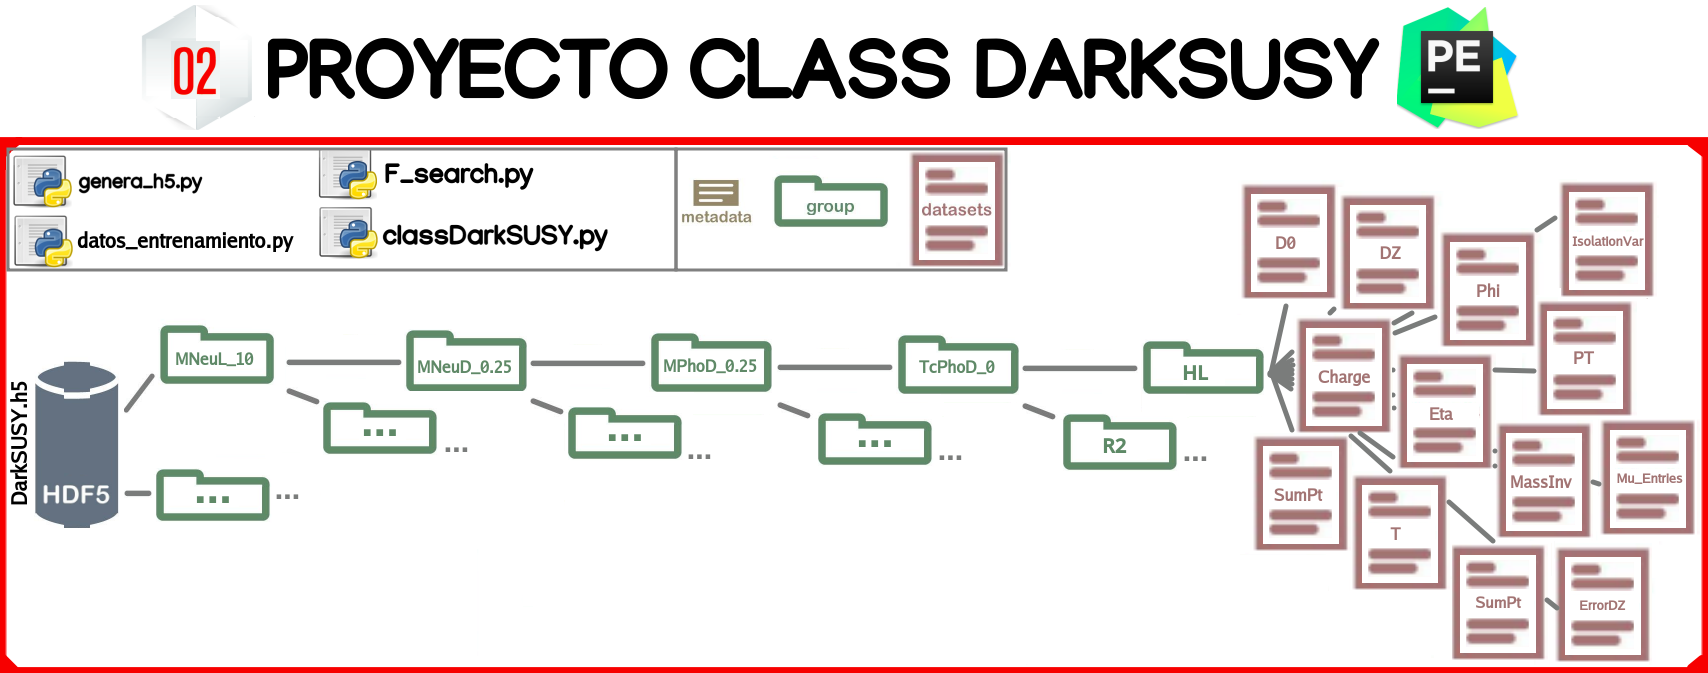
\includegraphics[width=1\textwidth]{Cap3/imagenes/class_darksusy.png}
\caption[Estructura del proyecto interpretador de la información contenida en los archivos $\textsf{*.root}$.]{Estructura del proyecto interpretador de la información contenida en los archivos $\textsf{*.root}$\footnote{Página del proyecto: \href{https://github.com/franky8939/DarkSUSY/blob/master/00-Convertidores/genera_h5.py}{https://github.com/franky8939/\-Dark\-SUSY/\-blob/\-mas\-ter/\-00-\-Con\-ver\-ti\-do\-res/\-ge\-ne\-ra\_h5.\-py}.}. }
\label{class_darksusy1}
\end{figure}
\footnotetext{Página del proyecto: \href{https://github.com/franky8939/DarkSUSY/blob/master/modules/darkSUSY/classDarkSUSY.py}{https://\-github\-.com/\-franky8939/\-DarkSUSY/\-blob/\-master/\-modules/\-darkSUSY/\-class\-Dark\-SUSY.\-py}}

\begin{table}[!t]
\small
\centering
\begin{tabular}{|p{.12\textwidth}p{.09\textwidth}p{.09\textwidth}p{.6\textwidth}|}
\toprule
Notación & Notación & Particula & Definición\\
$\textsf{python}$ & $\textsf{x}_j$ &  & \\ 
\midrule
$\textsf{MassInv}$ & $m$ & $n_1$,    $n_D$, $\gamma_D,~ \mu$ & Masa invariante\\
$\textsf{PT}$ & $P_{T}$ & $\mu$, $\gamma_D$ & Momento en dirección transversal de la partícula.\\
$\textsf{Eta}$ & $\eta$ & $\mu$, $\gamma_D$ & Pseudoapidez, esta representa la coordenada espacial que describe el ángulo de una partícula en relación con el eje del haz. \\
$\textsf{Phi}$ & $\phi$ &  $\mu$, $\gamma_D$ & Ángulo azimutal.\\
$\textsf{T}$ & $c\tau$ &  $\mu$, $\gamma_D$  & Tiempo de vida media, esta describe la descomposición de las partículas, se expresa comúnmente en términos de vida media, constante de descomposición o vida media. \\
$\textsf{D0}$ & $D_0$ &  $\mu$, $\gamma_D$  & Parámetro de impacto transversal, se define como la distancia transversal al eje del haz en el punto de máxima aproximación, donde su signo esta dado de acuerdo al momento angular de la traza alrededor de eje.\\
$\textsf{Dz}$ & $D_Z$ & $\mu$, $\gamma_D$   & Parámetro de impacto longitudinal, definido como la posición de la coordenada $z$ de la traza en el punto de maximo acercamiento.\\
$\textsf{SumPt}$ & $\textsf{Sum}P_T$ & $\mu$  & Variable de aislamiento basada en el rastreador de partículas, se define como la suma escalar del $P_T$ de las partículas en el plano $\eta \times \phi$ dentro de un cono $\Omega$(ver Fig. \ref{torre}a). Solo existen para $k=\textsf{CMS},  \textsf{HL}$. \\
$\textsf{IsolationVar}$ & $Iso$ & $\mu$ & Combinación del aislamiento de \textbf{ECAL}, \textbf{HCAL} (ver sección \ref{Experimento_CMS}) y $\textsf{Sum}P_T$. Solo existen para $k=\textsf{CMS},  \textsf{HL}$.\\

%\item[-] \texttt{SumPtNeutral}: xxx\\
%\item[-] \texttt{SumPtCharged}: xxx\\
\bottomrule
\end{tabular}
\caption{Algunas propiedades con sus definiciones de las partículas usadas en la investigación.}
\label{propiedades}
\end{table}

Dada la gran cantidad de información y archivos a procesar para el análisis estadístico incluso ante un acceso eficiente, la gran dispersión de la información hace que los procesos de recolección de datos sea lento y con altos requerimientos de memoria, la forma en que se abordo esta dificultad fue incorporar la información solicitada en un mismo archivo de tipo \textbf{HDF5} (\textbf{H}ierarchical \textbf{D}ata \textbf{F}ormat) la cual posee una librería de propósito general con un formato de ficheros para el almacenamiento de datos científicos, ver Fig. \ref{class_darksusy1}. Algunas de las propiedades que serán guardadas como motivos de esta investigación se encuentran las definidas en la Tabla \ref{propiedades}, donde $\textsf{x}_j$ hace referencia a la propiedad de interés, estás se pueden ver en la Tabla \ref{propiedades}.

%\begin{figure}[!h]
%\centering
%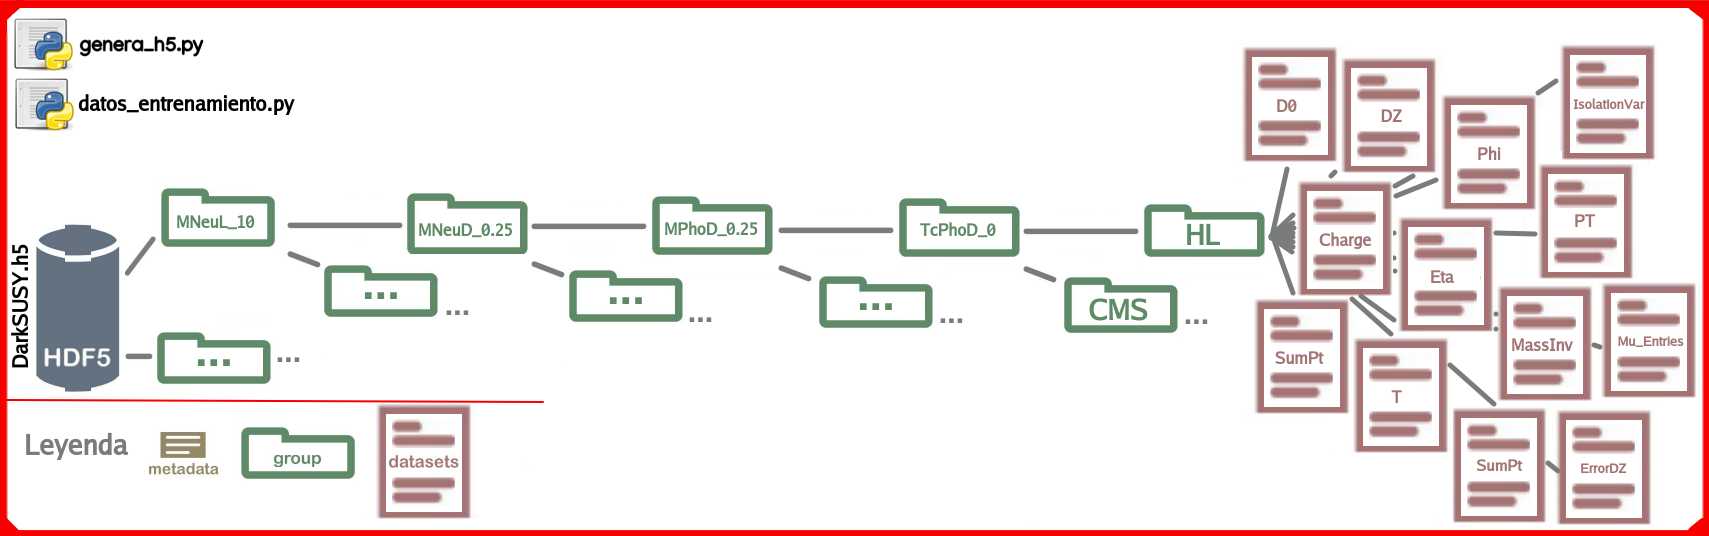
\includegraphics[width=1\textwidth]{Simulacion/imagenes/class_darksusy3.png}
%\caption[Estructura de los metadatos con la información filtrada.]{Estructura de los metadatos con la información filtrada\footnotemark.}
%\label{class_darksusy2}
%\end{figure}
%Este formato de datos \textbf{HDF5} fue creado para atender las necesidades de científicos e ingenieros que trabajan en entornos de computación de altas prestaciones que requieran un uso intensivo de datos, de aquí que este predeterminado para que sea muy eficiente en el almacenaniento y el acceso. 